\let\negmedspace\undefined
\let\negthickspace\undefined
\documentclass[journal]{IEEEtran}
\usepackage[a5paper, margin=10mm, onecolumn]{geometry}
%\usepackage{lmodern} % Ensure lmodern is loaded for pdflatex
\usepackage{tfrupee} % Include tfrupee package

\setlength{\headheight}{1cm} % Set the height of the header box
\setlength{\headsep}{0mm}     % Set the distance between the header box and the top of the text

\usepackage{gvv-book}
\usepackage{gvv}
\usepackage{cite}
\usepackage{amsmath,amssymb,amsfonts,amsthm}
\usepackage{algorithmic}
\usepackage{graphicx}
\usepackage{textcomp}
\usepackage{xcolor}
\usepackage{txfonts}
\usepackage{listings}
\usepackage{enumitem}
\usepackage{mathtools}
\usepackage{gensymb}
\usepackage{comment}
\usepackage[breaklinks=true]{hyperref}
\usepackage{tkz-euclide} 
\usepackage{listings}
% \usepackage{gvv}                                        
\def\inputGnumericTable{}                                 
\usepackage[latin1]{inputenc}                                
\usepackage{color}                                            
\usepackage{array}                                            
\usepackage{longtable}                                       
\usepackage{calc}                                             
\usepackage{multirow}                                         
\usepackage{hhline}                                           
\usepackage{ifthen}                                           
\usepackage{lscape}
\begin{document}

\bibliographystyle{IEEEtran}
\vspace{3cm}

\title{1.1.5.33}
\author{EE24BTECH11059 - Yellanki Siddhanth
}
% \maketitle
% \newpage
% \bigskip
{\let\newpage\relax\maketitle}

\renewcommand{\thefigure}{\theenumi}
\renewcommand{\thetable}{\theenumi}
\setlength{\intextsep}{10pt} % Space between text and floats


\numberwithin{equation}{enumi}
\numberwithin{figure}{enumi}
\renewcommand{\thetable}{\theenumi}


\textbf{Question}:\\

The vectors $\lambda\hat{i} + \hat{j} +2\hat{k}$, $\hat{i} + \lambda\hat{j} - \hat{k}$ and $2\hat{i} - \hat{j} +\lambda\hat{k}$  are coplanar if $\lambda = $
\\ \textbf{Solution: }\\
    \begin{table}[h!]    
      \centering
      

      \caption{}
    \end{table}\\
The rank of a matrix $M$ is less than 3, then the matrix is coplanar. 
    \begin{align}
        Rank\brak{M} = 2\label{eq1.1.6.19.1}
    \end{align}
Equivalently,
    \begin{align}
        \abs{M} = 0 \label{eq1.1.6.19.2}
    \end{align}
    \begin{align}
        \abs{M} = \myvec{\lambda & 1 & 2 \\ 1 & \lambda & -1 \\ 2 & -1 & \lambda} = 0 \label{eq1.1.6.19.3}
    \end{align}
    \begin{align}
        \lambda\brak{\lambda^2 - 1} - 1\brak{\lambda+2} + 2\brak{-1-2\lambda} = 0  \label{eq1.1.6.19.4}
    \end{align}
    \begin{align}
        \lambda^3 - 6\lambda - 4 = 0  \label{eq1.1.6.19.5}
    \end{align}
    \begin{align}
        \brak{\lambda + 2}\brak{\lambda^2 - 2\lambda - 2} = 0  \label{eq1.1.6.19.6}
    \end{align}
    \begin{align}
         \lambda = -2 \text{ or } \lambda = 1 \pm \sqrt{3}\label{eq1.1.6.19.6}
    \end{align}
    
$\therefore$ Verifying $\lambda$ values:
    \begin{figure}[h]
        \centering
       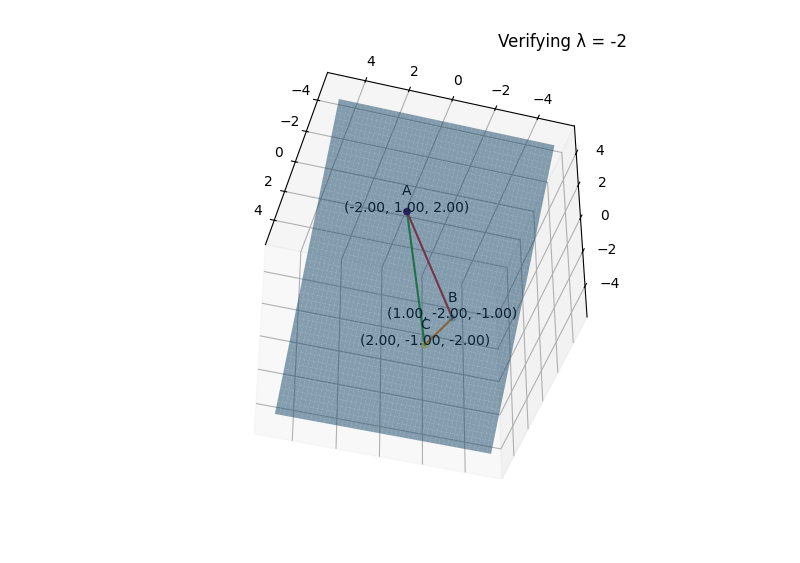
\includegraphics[width=0.7\linewidth]{figs/fig1.png}
       \caption{}
       \label{graph}
    \end{figure}
    \begin{figure}[h]
        \centering
       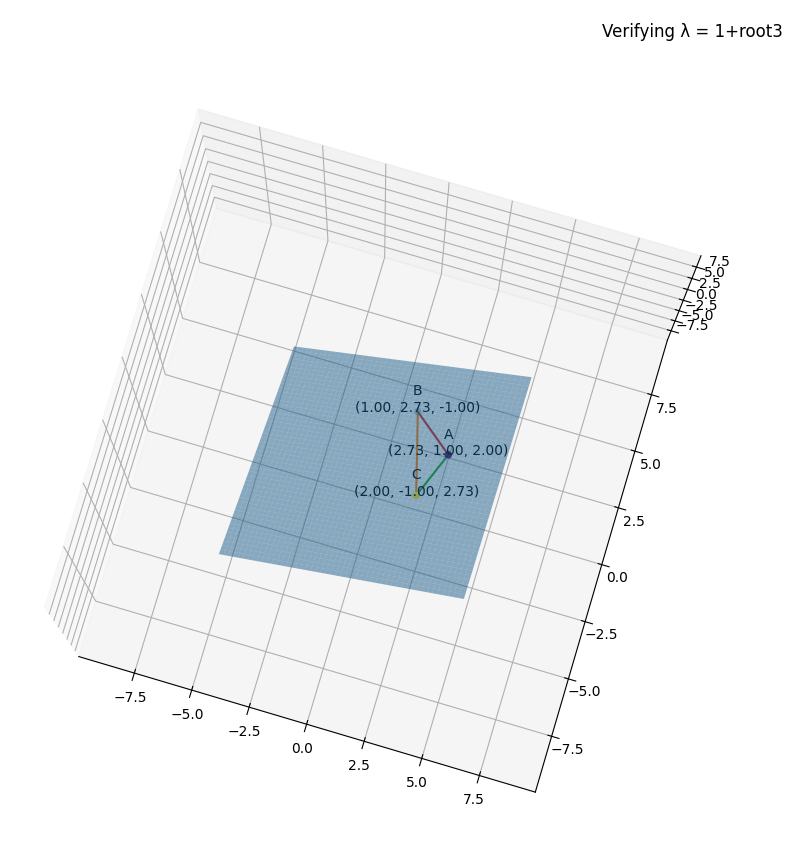
\includegraphics[width=0.7\linewidth]{figs/fig2.png}
       \caption{}
       \label{graph}
    \end{figure}
    \begin{figure}[h]
        \centering
       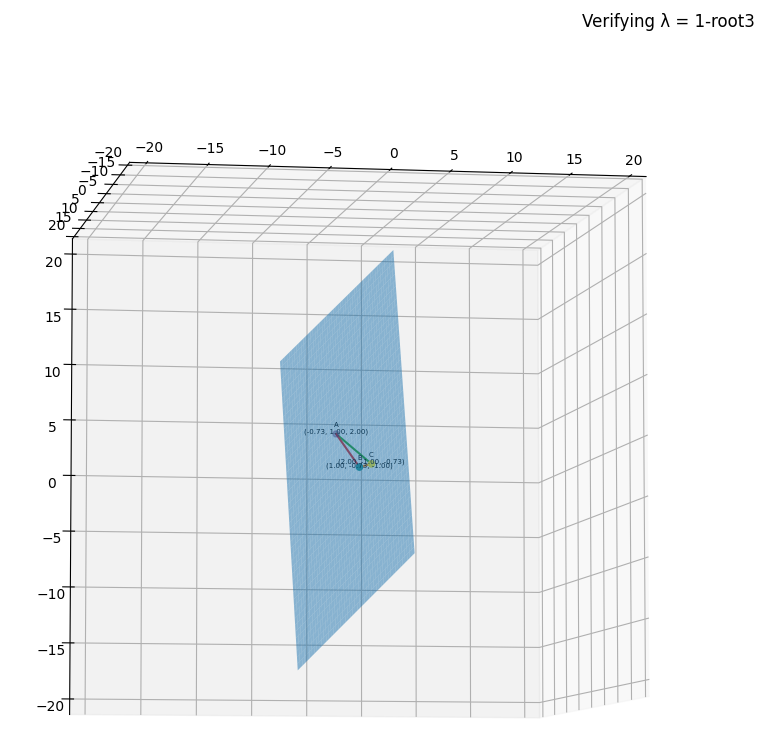
\includegraphics[width=0.7\linewidth]{figs/fig3.png}
       \caption{}
       \label{graph}
    \end{figure}
\end{document}  





